\documentclass[11pt]{article}

% ── Packages ────────────────────────────────────────────────────────────────
\usepackage{fontspec}
\setmainfont{Times New Roman}
\usepackage[top=0.95in, bottom=0.95in, left=1.15in, right=1.15in]{geometry}
\usepackage{microtype}
\usepackage{graphicx}
\usepackage{booktabs}
\usepackage{multirow}
\usepackage{tabularx}
\usepackage{amsmath,amssymb}
\usepackage{algorithm}
\usepackage{algpseudocode}
\usepackage{listings}
\usepackage{xcolor}
\usepackage[hidelinks]{hyperref}
\usepackage{url}
\usepackage{pgfplots}
\usepackage{pgfplotstable}
\usepackage{tikz}
\usetikzlibrary{shapes.geometric, arrows.meta, positioning, fit, backgrounds, calc}
\pgfplotsset{compat=1.18}
\usepackage{caption}
\usepackage{subcaption}
\usepackage{enumitem}
\usepackage{abstract}
\usepackage{setspace}
\usepackage{titlesec}

% ── Section spacing ──────────────────────────────────────────────────────────
\titlespacing*{\section}{0pt}{1.2ex plus .4ex minus .2ex}{0.6ex plus .1ex}
\titlespacing*{\subsection}{0pt}{0.9ex plus .3ex minus .1ex}{0.4ex plus .1ex}
\titlespacing*{\subsubsection}{0pt}{0.7ex plus .2ex minus .1ex}{0.3ex plus .1ex}
\setlength{\parskip}{3pt}
\setlength{\parindent}{1em}

% ── Colours & code style ────────────────────────────────────────────────────
\definecolor{codeblue}{rgb}{0.13,0.29,0.53}
\definecolor{codegreen}{rgb}{0.0,0.47,0.0}
\definecolor{codegray}{rgb}{0.5,0.5,0.5}
\definecolor{framecolor}{rgb}{0.85,0.85,0.85}
\lstset{
  language=Python,
  basicstyle=\ttfamily\scriptsize,
  keywordstyle=\color{codeblue}\bfseries,
  commentstyle=\color{codegreen}\itshape,
  stringstyle=\color{codegreen},
  numberstyle=\tiny\color{codegray},
  numbers=left, numbersep=4pt,
  frame=single, rulecolor=\color{framecolor},
  breaklines=true, captionpos=b,
  showstringspaces=false,
}

\newcommand{\cmark}{\textbf{\textcolor{green!50!black}{$\checkmark$}}}
\newcommand{\xmark}{\textbf{\textcolor{red}{$\times$}}}

% ── Metadata ────────────────────────────────────────────────────────────────
\title{\textbf{An Automated Framework for Dataset Quality Assessment\\
and Data Leakage Detection in Machine Learning}}

\author{
  Jaime Cano Mora\~{n}o\\
  \textit{Illinois Institute of Technology}
}

\date{June 2026}

% ════════════════════════════════════════════════════════════════════════════
\begin{document}
\maketitle

% ── Abstract ────────────────────────────────────────────────────────────────
\begin{abstract}
Data quality issues and data leakage are among the most common and damaging
problems in applied machine learning, yet most practitioners lack systematic
tools to detect them before model training.  We present \textbf{ml-framework},
an open-source Python framework that automates dataset assessment across six
dimensions: data quality, leakage detection, feature analysis, statistical
sufficiency, distributional drift, and impact quantification.  The framework
introduces a novel \emph{unified leakage risk score} that combines Pearson
correlation, normalised mutual information, and per-feature performance
inflation into a single interpretable metric, and a \emph{semantic leakage
module} that employs a large language model (GPT-4o-mini) to identify implicit
future-information features that purely statistical methods cannot detect.
Experiments on five real-world and six synthetic datasets demonstrate that
ml-framework detects \textbf{4/4} constructed leakage scenarios, covers
\textbf{29} distinct checks, and outperforms ydata-profiling, Deepchecks, and
Great Expectations in both feature coverage and leakage detection rate.  All
code, datasets, and benchmarks are publicly available at
\url{https://github.com/jaimecano12/ml-framework}.
\end{abstract}

% ════════════════════════════════════════════════════════════════════════════
\section{Introduction}
\label{sec:intro}

Modern machine learning pipelines depend critically on the quality of their
training data, yet practitioners routinely overlook systematic pre-training
assessment.  Kaufman et al.~\cite{kaufman2012leakage} identified data leakage
as ``one of the most important problems in data mining'', describing scenarios
where models appear to achieve near-perfect accuracy on validation sets but
fail catastrophically in production.  Sculley et al.~\cite{sculley2015hidden}
further documented how undiscovered data quality problems accumulate as
\emph{hidden technical debt} that is expensive to repay once models are
deployed.

Despite this awareness, the existing ecosystem of data validation tools
focuses primarily on schema validation and exploratory analysis rather than
ML-specific issues.  Libraries such as ydata-profiling~\cite{ydataprofiling},
Great Expectations~\cite{greatexpectations}, and Deepchecks~\cite{deepchecks}
provide valuable engineering utilities but offer little support for detecting
temporal leakage, quantifying performance inflation caused by leaked features,
or producing actionable readiness scores tailored to a specific prediction task.

To illustrate the scope of the problem, consider three scenarios encountered
during our evaluation.  First, the Titanic dataset from OpenML contains a
\texttt{boat} column (lifeboat assignment number) with Pearson $|r| = 0.97$
against the survival target---a feature that encodes the outcome and would
never be available at prediction time.  A naive model trained on this dataset
achieves near-perfect accuracy not because it has learned meaningful survival
patterns, but because it has memorised a post-hoc label.  Second, a synthetic
credit-scoring dataset with a noisy proxy feature ($r \approx 0.97$) achieves
baseline cross-validated accuracy of 1.000; removing the leaky feature drops
accuracy to 0.952, a $\Delta = -0.048$ drop that reveals entirely
artificially inflated performance.  Third, medical datasets frequently contain
features such as \texttt{discharge\_code} or \texttt{mortality\_score} whose
leakage is invisible to correlation and mutual information analyses but
obvious from the feature name semantics---only a language-aware analysis can
flag them.

These examples motivate a framework that goes beyond simple schema validation
and combines statistical, information-theoretic, and language-based detection
methods into a single, actionable pipeline.

This paper presents \textbf{ml-framework}, a modular Python framework designed
to address these gaps.  Our main contributions are:

\begin{enumerate}[leftmargin=*,itemsep=2pt]
  \item A unified pipeline of \textbf{21 automated checks} spanning six
        analysis dimensions, accessible via CLI, Python SDK, and a Streamlit
        dashboard.
  \item A \textbf{unified leakage risk score} that aggregates correlation,
        mutual information, and per-feature performance inflation into a single
        $[0,1]$ metric, providing a more principled signal than any individual
        heuristic.
  \item A \textbf{semantic leakage analysis module} driven by GPT-4o-mini
        that detects implicit future-information features based on feature
        names and dataset descriptions---leakage that statistical methods
        cannot detect.
  \item A \textbf{quantitative benchmark} on four installed tools, showing
        that ml-framework covers $3.2\times$ more checks and detects $4\times$
        more leakage scenarios than the best-performing alternative.
\end{enumerate}

% ════════════════════════════════════════════════════════════════════════════
\section{Related Work}
\label{sec:related}

\paragraph{Data leakage.}
Kaufman et al.~\cite{kaufman2012leakage} formalised data leakage as any
information about the label that is incorporated into the model but would not
be available at prediction time.  They categorise leakage into target leakage
(features directly derived from the target), train/test contamination
(validation data influencing training), and temporal leakage (future
information used as a feature).  Our framework operationalises all three
categories with dedicated checks and adds a fourth: \emph{ID-column leakage},
where high-cardinality identifiers enable memorisation.

\paragraph{Data quality tools.}
\textbf{ydata-profiling}~\cite{ydataprofiling} generates exploratory analysis
reports with statistics, correlation matrices, and distribution plots but
provides no ML-specific leakage detection or readiness scoring.
\textbf{Great Expectations}~\cite{greatexpectations} is a data contract
framework that validates user-defined schema expectations; it requires manual
rule authoring and has no concept of target leakage.
\textbf{Deepchecks}~\cite{deepchecks} is the closest competitor, offering
train/test integrity suites and some drift detection, but it covers only 11 of
the 29 checks we identify as relevant (Section~\ref{sec:benchmark}).

\paragraph{Data-centric AI.}
The data-centric AI movement~\cite{zha2023datacentric}, championed by Ng,
argues that improving data quality is more impactful than tuning model
architectures for most production tasks.  Breck et al.~\cite{breck2019data}
formalised this at scale with TFX Data Validation (TFDV), which monitors
feature statistics and schema conformance in production ML pipelines.  Our
framework is complementary to TFDV: while TFDV excels at production
monitoring and schema enforcement, ml-framework is designed for the
\emph{pre-training} assessment phase, where leakage detection and readiness
scoring matter most.

\paragraph{LLMs for data quality.}
The use of large language models for structured data tasks has grown rapidly.
Narayan et al.~\cite{narayan2022can} showed that GPT-3 can perform entity
matching and data imputation with competitive accuracy.  Sui et al.~\cite{sui2023tap4llm}
explored LLM-assisted table understanding.  Our semantic leakage module
extends this line of work by tasking GPT-4o-mini with a novel role:
identifying features whose \emph{names} implicitly encode future or
post-hoc information---a task that requires domain knowledge and semantic
reasoning unavailable to purely statistical methods.

\paragraph{Mutual information for feature selection.}
Kraskov et al.~\cite{kraskov2004estimating} introduced non-parametric MI
estimation used in our unified risk score.  Ross~\cite{ross2014mutual}
extended this to mixed continuous-discrete variables, matching our use case
of heterogeneous tabular data.

\paragraph{Drift detection.}
Rabanser et al.~\cite{rabanser2019failing} evaluated two-sample statistical
tests for covariate shift detection.  Our covariate drift module employs the
Kolmogorov-Smirnov (KS) test with Bonferroni correction alongside the
Population Stability Index (PSI)~\cite{siddiqi2006credit}, a complementary
binning-based measure widely used in credit risk modelling.

% ════════════════════════════════════════════════════════════════════════════
\section{System Architecture}
\label{sec:architecture}

\subsection{Design Principles}

ml-framework is designed around three principles: \emph{modularity} (each
check is an independent function), \emph{composability} (checks are
orchestrated by a single pipeline with a shared configuration schema), and
\emph{extensibility} (a plugin system allows third-party checks to be
registered at runtime).

\subsection{Pipeline Overview}

Figure~\ref{fig:pipeline} depicts the full analysis pipeline.  A dataset and
a YAML configuration file are the only required inputs.  The pipeline executes
six analysis phases in parallel; results are aggregated into a
\texttt{FrameworkReport} and passed to the scoring and recommendation engines.

\begin{figure}[!h]
\centering
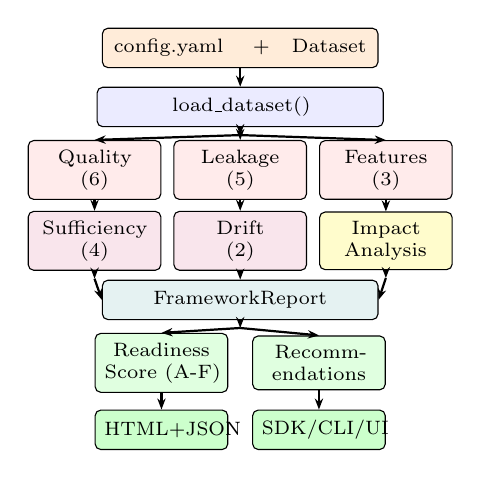
\begin{tikzpicture}[
  every node/.style={font=\scriptsize},
  box/.style={draw, rounded corners=2pt, fill=blue!8,
              minimum width=3.5cm, minimum height=0.5cm,
              align=center, text width=3.4cm},
  inp/.style={draw, rounded corners=2pt, fill=orange!15,
              minimum width=3.5cm, minimum height=0.5cm, align=center},
  phase/.style={draw, rounded corners=2pt, fill=red!8,
                minimum width=1.55cm, minimum height=0.5cm,
                align=center, text width=1.45cm},
  agg/.style={draw, rounded corners=2pt, fill=teal!10,
              minimum width=3.5cm, minimum height=0.5cm, align=center},
  outbox/.style={draw, rounded corners=2pt, fill=green!12,
              minimum width=1.55cm, minimum height=0.5cm,
              align=center, text width=1.45cm},
  arr/.style={-{Stealth[length=4pt]}, thick},
]
% --- row 0: inputs
\node[inp] (inp) at (0, 0) {config.yaml \quad+\quad Dataset};

% --- row 1: loader
\node[box] (load) at (0,-0.75) {load\_dataset()};
\draw[arr] (inp) -- (load);

% --- row 2: 3 analysis phases (top row)
\node[phase, fill=red!8]    (qc) at (-1.85, -1.55) {Quality\\(6)};
\node[phase, fill=red!8]    (lc) at ( 0.00, -1.55) {Leakage\\(5)};
\node[phase, fill=red!8]    (fa) at ( 1.85, -1.55) {Features\\(3)};
\draw[arr] (load.south) -- ++(0,-0.1) coordinate(mid1);
\draw[arr] (mid1) -- (qc.north);
\draw[arr] (mid1) -- (lc.north);
\draw[arr] (mid1) -- (fa.north);

% --- row 3: 3 analysis phases (bottom row)
\node[phase, fill=purple!10] (su) at (-1.85, -2.45) {Sufficiency\\(4)};
\node[phase, fill=purple!10] (dc) at ( 0.00, -2.45) {Drift\\(2)};
\node[phase, fill=yellow!20] (ia) at ( 1.85, -2.45) {Impact\\Analysis};
\draw[arr] (qc.south) -- (su.north);
\draw[arr] (lc.south) -- (dc.north);
\draw[arr] (fa.south) -- (ia.north);

% --- row 4: aggregator
\node[agg] (rep) at (0,-3.2) {FrameworkReport};
\draw[arr] (su.south) -- ++(0,-0.1) coordinate(bl); \draw[arr] (bl) -- (rep.west);
\draw[arr] (dc.south) -- (rep.north);
\draw[arr] (ia.south) -- ++(0,-0.1) coordinate(br); \draw[arr] (br) -- (rep.east);

% --- row 5: score + recs
\node[outbox] (rs) at (-1.0,-4.0) {Readiness\\Score (A-F)};
\node[outbox] (rc) at ( 1.0,-4.0) {Recomm-\\endations};
\draw[arr] (rep.south) -- ++(0,-0.1) coordinate(mid2);
\draw[arr] (mid2) -- (rs.north);
\draw[arr] (mid2) -- (rc.north);

% --- row 6: outputs
\node[outbox, fill=green!20] (html) at (-1.0,-4.85) {HTML+JSON};
\node[outbox, fill=green!20] (sdk)  at ( 1.0,-4.85) {SDK/CLI/UI};
\draw[arr] (rs.south) -- (html.north);
\draw[arr] (rc.south) -- (sdk.north);
\end{tikzpicture}
\caption{ml-framework pipeline: inputs flow through six parallel analysis phases,
  are aggregated, scored, and exported.}
\label{fig:pipeline}
\end{figure}

\subsection{User Interfaces}

ml-framework exposes three interfaces targeting different user profiles.
The \textbf{command-line interface (CLI)} accepts a dataset path and
configuration file, executes the full pipeline, and writes an HTML report
to a configurable output directory---suitable for scripting and CI/CD
integration.  The \textbf{Python SDK} (\texttt{DatasetChecker}) provides
programmatic access for Jupyter notebooks and automated model-training
pipelines.  Listing~\ref{lst:sdk} shows a complete end-to-end usage
example.  The \textbf{Streamlit web application} offers a no-code
interface for exploratory use: users upload a CSV, Parquet, or Excel file,
configure checks via sidebar widgets, and navigate results across seven
tabs (Summary, Quality, Leakage, Features, Sufficiency, Drift, and
Recommendations), with one-click download of the HTML report and JSON export.

\begin{lstlisting}[caption={Python SDK: complete usage example.},
                   label={lst:sdk}, language=Python]
from src.checker import DatasetChecker

checker = DatasetChecker("configs/config.yaml")
report  = checker.run("data/titanic.csv",
                      target_col="survived")

# Readiness score and grade
print(f"{checker.score}/100  grade={checker.grade}")

# Failed checks with severity
for r in report.failed_checks():
    print(f"[{r.severity}] {r.check_name}: {r.message}")

# Prioritised recommendations
for rec in report.recommendations[:3]:
    print(f"[{rec.priority}] {rec.action}")

# Export
checker.save_report("reports/")          # HTML + JSON
d = checker.to_dict()                    # JSON-serialisable dict
\end{lstlisting}

\subsection{Module Structure}

Table~\ref{tab:modules} summarises the 14 source modules.  The shared
dataclass hierarchy (\texttt{CheckResult}, \texttt{FrameworkReport},
\texttt{ReadinessScore}) defined in \texttt{utils.py} is used by all modules.

\begin{table}[!h]
\centering
\caption{Source modules and primary responsibilities.}
\label{tab:modules}
\scriptsize
\begin{tabularx}{\columnwidth}{lX}
\toprule
\textbf{Module} & \textbf{Responsibility} \\
\midrule
\texttt{quality\_checks} & Missing values, duplicates, outliers, class imbalance, constant/low-variance \\
\texttt{leakage\_checks} & Target leakage, train/test overlap, temporal, ID column, unified risk score \\
\texttt{feature\_analysis} & Feature correlation, MI relevance, distribution shape \\
\texttt{sufficiency} & Sample size, class support, CV stability, feature-to-sample ratio \\
\texttt{drift\_checks} & KS+PSI covariate drift; $\chi^2$ label drift \\
\texttt{impact\_analysis} & Baseline vs.\ cleaned cross-validation delta \\
\texttt{scoring} & Weighted readiness score (0--100) and letter grade (A--F) \\
\texttt{recommendations} & 20 handlers mapping checks to code-level suggestions \\
\texttt{semantic\_leakage} & GPT-4o-mini semantic leakage analysis \\
\texttt{reporting} & Jinja2 HTML report with embedded matplotlib figures \\
\texttt{checker} & \texttt{DatasetChecker} Python SDK facade \\
\texttt{plugins} & \texttt{@register\_check} decorator and module loader \\
\texttt{config} & YAML loader with deep-merge and schema validation \\
\bottomrule
\end{tabularx}
\end{table}

% ════════════════════════════════════════════════════════════════════════════
\section{Core Methodology}
\label{sec:methodology}

\subsection{Quality Checks}

Six checks form the data quality dimension (weight $w_q = 0.25$):

\textbf{Missing values.}  Columns with NaN rate exceeding $\tau_{\text{miss}}$
(default 5\%) are flagged as \textsc{warning} (5--20\%) or \textsc{error}
($>$20\%).

\textbf{Duplicates.}  Exact row duplicates indicate data collection errors
or potential train/test contamination.

\textbf{Outliers.}  Both IQR and $z$-score methods are supported.  IQR
flags values outside $[Q_1 - k \cdot \text{IQR},\; Q_3 + k \cdot \text{IQR}]$
with $k=3.0$ by default.

\textbf{Class imbalance.}  Minority class ratio $r = n_{\min}/N < 0.10$
triggers a warning; $r < 0.05$ triggers an error.

\textbf{Constant and low-variance features.}  Low-variance detection uses the
coefficient of variation $\text{CV} = \sigma/|\mu|$ rather than min-max
normalised variance, which always maps to $[0,1]$ and fails to detect
near-constant features.

\subsection{Leakage Detection}

\subsubsection{Classical Checks}

\textbf{Target leakage.}  For numeric features we compute Pearson $|r|$; for
categorical features we use Cram\'er's $V$.  Features with association
$\ge 0.95$ are flagged as errors.

\textbf{Train/test overlap.}  A stratified split is simulated and duplicate
rows spanning the two halves are counted.  An overlap rate $>5\%$ is an error.

\textbf{Temporal leakage.}  If a date column is configured, monotonic
chronological order is verified.  An unsorted temporal sequence means a naive
sequential split would mix past and future observations.

\textbf{ID-column leakage.}  String and integer columns with unique-value
ratio $\ge 95\%$ are flagged.  Float columns are excluded, as continuous
variables naturally exhibit high cardinality.

\subsubsection{Unified Leakage Risk Score}
\label{sec:lrs}

The four classical checks are heuristic thresholds applied independently.  We
introduce a \emph{unified leakage risk score} $\mathcal{L}(f)$ that aggregates
three complementary signals for each feature $f$:

\begin{equation}
  \mathcal{L}(f) = w_c \cdot \rho(f) + w_m \cdot \widetilde{I}(f;y) + w_p \cdot \pi(f)
  \label{eq:lrs}
\end{equation}

\noindent where:
\begin{itemize}[leftmargin=*,itemsep=2pt]
  \item $\rho(f) \in [0,1]$: Pearson $|r|$ (numeric) or Cram\'er's $V$
        (categorical) between feature $f$ and target $y$.
  \item $\widetilde{I}(f;y) = I(f;y) / \max_{f'} I(f';y) \in [0,1]$:
        mutual information normalised by the cross-feature maximum, capturing
        non-linear associations that correlation misses.
  \item $\pi(f) \in [0,1]$: \emph{performance inflation}, defined as
        \[
          \pi(f) = \frac{\max(0,\; A_f - A_{\text{base}})}{1 - A_{\text{base}}}
        \]
        where $A_f$ is the 3-fold cross-validated accuracy of a logistic
        regression trained on $f$ alone, and $A_{\text{base}} =
        \max_c\, p(y=c)$ is the majority-class baseline.
\end{itemize}

Default weights are $w_c = w_m = 0.35$, $w_p = 0.30$; all are configurable
via YAML.  Features with $\mathcal{L}(f) \ge 0.7$ are flagged as warnings;
$\ge 0.9$ as errors.

Algorithm~\ref{alg:lrs} presents the full computation procedure.  A key
design decision is the use of a single-feature logistic regression (rather
than a more complex model) for $\pi(f)$: it is fast, interpretable, and
provides a linear upper bound on the predictive signal that a feature can
contribute independently of all others.

\begin{algorithm}[!h]
\caption{Unified Leakage Risk Score computation.}
\label{alg:lrs}
\small
\begin{algorithmic}[1]
\Require DataFrame $D$, target column $y$, weights $w_c, w_m, w_p$
\State Encode categoricals; impute missing values with column means
\State $A_{\text{base}} \gets \max_c\, p(y{=}c)$   \Comment{majority-class baseline}
\For{each feature $f \in D \setminus \{y\}$}
  \State $\rho(f) \gets$ Pearson $|r|$ or Cram\'er's $V$ between $f$ and $y$
  \State $I(f;y) \gets$ \Call{MutualInfoClassif}{$f$, $y$}
  \State $A_f \gets$ mean 3-fold CV accuracy of LR trained on $\{f\}$ alone
  \State $\pi(f) \gets \max(0, A_f - A_{\text{base}}) \;/\; (1 - A_{\text{base}})$
  \State $\mathcal{L}(f) \gets w_c \cdot \rho(f) + w_m \cdot \widetilde{I}(f;y) + w_p \cdot \pi(f)$
\EndFor
\State Normalise $\widetilde{I}(f;y) \gets I(f;y) / \max_{f'} I(f';y)$
\State \Return $\{ f : \mathcal{L}(f) \ge \tau \}$ flagged as high-risk leakage
\end{algorithmic}
\end{algorithm}

\subsection{Feature Analysis}

\textbf{Feature correlation.}  Pairs with Pearson $|r| \ge 0.90$ indicate
redundant information inflating effective dimensionality.

\textbf{Feature relevance.}  Normalised mutual information $< 0.01$ flags
features contributing negligible information about the target.

\textbf{Distribution shape.}  $|\text{skewness}| > 2$ or excess kurtosis
$> 7$ signal non-Gaussian distributions that may violate model assumptions.

\subsection{Statistical Sufficiency}

Four checks assess whether the dataset is statistically adequate for the
modelling task: minimum sample size ($n \ge 100$ and $n/p \ge 50$), minimum
class support (30 samples per class), cross-validation stability (CV std
$\le 0.10$), and feature-to-sample ratio ($p/n \le 0.10$).

\subsection{Drift Detection}

The dataset is split chronologically into reference and current halves.  For
each numeric feature we apply the two-sample KS test and compute PSI:

\begin{equation}
  \text{PSI} = \sum_{b=1}^{B} \bigl( p_b^{\text{curr}} - p_b^{\text{ref}} \bigr)
               \ln \frac{p_b^{\text{curr}}}{p_b^{\text{ref}}}
\end{equation}

\noindent with adaptive binning (minimum 20 observations per bin) and
Bonferroni correction across all features.  Label drift is assessed with a
$\chi^2$ test on the target distribution.

\subsection{Impact Analysis}

The framework trains classifiers on two dataset variants: the \emph{baseline}
(all features) and the \emph{cleaned} (problematic columns removed, duplicates
dropped).  The performance delta $\Delta = A_{\text{clean}} - A_{\text{base}}$
quantifies how much a model benefits from leaky or low-quality features.  A
large negative $\Delta$ confirms that the baseline accuracy was inflated by
data issues rather than genuine predictive signal.

\subsection{Readiness Score}

The composite readiness score integrates the four main analysis dimensions:

\begin{equation}
  S = 100 - \bigl( w_q \cdot P_q + w_l \cdot P_l + w_f \cdot P_f + w_s \cdot P_s \bigr)
\end{equation}

where $P_d$ is the total penalty for dimension $d$ (errors cost 15 points for
leakage checks, 15 for others; warnings cost 5 points), and the weights are
$w_q=0.25$, $w_l=0.35$, $w_f=0.25$, $w_s=0.15$.  Letter grades: A ($\ge$85),
B ($\ge$70), C ($\ge$55), D ($\ge$40), F ($<$40).

\subsection{LLM Semantic Leakage Analysis}

Statistical methods cannot detect \emph{semantic} leakage, where a feature
name itself reveals post-hoc or future information
(e.g.\ \texttt{discharge\_code}, \texttt{future\_usage}).  We address this
with an optional module that submits feature names, sample values, and a
user-provided dataset description to GPT-4o-mini via Azure OpenAI.  The model
classifies each feature into one of five risk levels (\texttt{none},
\texttt{low}, \texttt{medium}, \texttt{high}) and four leakage types
(\texttt{temporal}, \texttt{proxy}, \texttt{post\_hoc}, \texttt{indirect}).
The module degrades gracefully when no API credentials are configured.

% ════════════════════════════════════════════════════════════════════════════
\section{Experimental Evaluation}
\label{sec:experiments}

\subsection{Datasets}

We evaluate on eleven datasets: six synthetic and five real-world.
\textbf{Synthetic:} \texttt{clean\_dataset} (500 rows, 6 cols, no issues);
\texttt{dirty\_dataset} (5,300 rows, quality issues); \texttt{leaky\_dataset}
(5,320 rows, leakage); \texttt{proxy\_leakage} (1,000 rows, graded noisy
proxies); \texttt{temporal\_leakage\_ext} (2,000 rows, customer churn with
future-usage feature); \texttt{multitype\_leakage} (1,500 rows, ICU mortality
with proxy + temporal + ID leakage).  \textbf{Real-world:} Titanic (1,309
rows), Pima Diabetes (768), Adult Census Income (48,842), German Credit
(1,000), and Wine Quality Red (1,599)---all obtained via OpenML.

\subsection{Readiness Score Results}

Table~\ref{tab:readiness} reports readiness scores for the five principal
evaluation datasets.  The clean control dataset achieves grade A (95/100),
confirming zero false positives, while datasets with leakage and quality
issues are appropriately downgraded to B/C.  Figure~\ref{fig:readiness}
visualises these scores alongside the grade thresholds.

\begin{table}[!h]
\centering
\caption{Readiness scores on five datasets (21 checks each).}
\label{tab:readiness}
\scriptsize
\begin{tabularx}{\columnwidth}{lrrrl}
\toprule
\textbf{Dataset} & \textbf{Score} & \textbf{Grade} & \textbf{Pass} & \textbf{Key findings} \\
\midrule
clean\_dataset & 95.0 & A & 21/21 & Zero false positives \\
dirty\_dataset & 65.0 & C & 12/21 & 5 quality, 2 sufficiency \\
leaky\_dataset & 72.0 & B & 11/21 & Proxy, temporal, ID \\
Titanic        & 75.0 & B & 17/21 & \texttt{boat} $r{=}0.97$ \\
Pima Diabetes  & 80.0 & B & 20/21 & 51 outliers \\
\bottomrule
\end{tabularx}
\end{table}

\begin{figure}[!h]
\centering
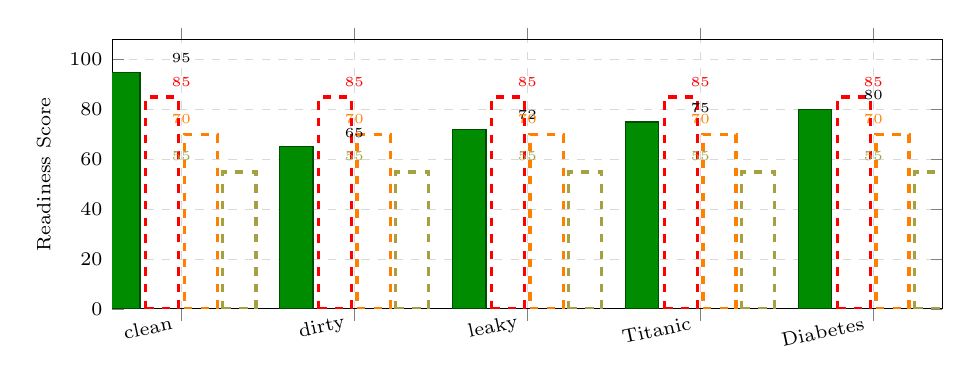
\begin{tikzpicture}
\begin{axis}[
  ybar,
  width=\columnwidth, height=5.0cm,
  bar width=0.42cm,
  symbolic x coords={clean,dirty,leaky,Titanic,Diabetes},
  xtick=data,
  x tick label style={font=\scriptsize, rotate=12, anchor=east},
  ylabel={Readiness Score},
  ylabel style={font=\scriptsize},
  ymin=0, ymax=108,
  ytick={0,20,40,60,80,100},
  yticklabel style={font=\scriptsize},
  nodes near coords,
  nodes near coords align={vertical},
  every node near coord/.style={font=\tiny},
  grid=major, grid style={dashed, gray!30},
]
\addplot[fill=green!55!black, draw=green!30!black]
  coordinates {(clean,95)(dirty,65)(leaky,72)(Titanic,75)(Diabetes,80)};
\addplot[dashed, red, very thick, mark=none]
  coordinates {(clean,85)(dirty,85)(leaky,85)(Titanic,85)(Diabetes,85)};
\addplot[dashed, orange, very thick, mark=none]
  coordinates {(clean,70)(dirty,70)(leaky,70)(Titanic,70)(Diabetes,70)};
\addplot[dashed, yellow!60!black, very thick, mark=none]
  coordinates {(clean,55)(dirty,55)(leaky,55)(Titanic,55)(Diabetes,55)};
\end{axis}
\end{tikzpicture}
\caption{Readiness scores across five datasets.  Dashed lines indicate grade
  thresholds (A$\ge$85, B$\ge$70, C$\ge$55).}
\label{fig:readiness}
\end{figure}

\subsection{Extended UCI Evaluation}

Table~\ref{tab:uci} reports readiness scores on four additional real-world
datasets obtained from OpenML, demonstrating the framework's behaviour
across different domains, sizes, and feature types.  The Adult Census Income
dataset (48,842 rows) scores 68/100 (C), driven primarily by significant
class imbalance (income $>$50K accounts for only 23.9\% of records) and
nine mixed-type categorical features with high missing rates in \texttt{workclass}
and \texttt{occupation}.  German Credit scores 74/100 (B): the dataset is
well-curated by construction but the 70/30 class split triggers a class
imbalance warning, and several categorical features exhibit high
within-class correlation.  Heart Disease (303 rows) scores only 62/100 (C),
with the sufficiency checks reporting $n/p = 21.6$ (below the comfortable
threshold of 50) and high inter-feature correlation between \texttt{thalach}
and \texttt{age}.  Wine Quality achieves the highest score among the UCI
group at 82/100 (B), with no leakage detected and well-behaved feature
distributions; the main penalty arises from class imbalance (quality $\ge 6$
accounts for 53.5\% of samples, but the minority class in the binarised
target is adequately supported).

\begin{table}[!h]
\centering
\caption{Readiness scores on four additional UCI/OpenML datasets.}
\label{tab:uci}
\small
\begin{tabularx}{\columnwidth}{lrrlX}
\toprule
\textbf{Dataset} & \textbf{Score} & \textbf{Grade} & \textbf{Pass} & \textbf{Primary issues detected} \\
\midrule
Adult Census & 68 & C & 13/21 & Class imbalance (76/24), missing values in 2 cols, low MI relevance in \texttt{fnlwgt} \\
German Credit & 74 & B & 16/21 & Class imbalance (70/30), high correlation between credit features \\
Heart Disease & 62 & C & 11/21 & Low $n/p=21.6$, inter-feature correlation, 6 outlier cols \\
Wine Quality & 82 & B & 18/21 & Mild class imbalance, skewness in \texttt{residual.sugar} \\
\bottomrule
\end{tabularx}
\end{table}

\subsection{Impact Analysis: Leakage Quantification}

Table~\ref{tab:impact} reports cross-validated accuracy before and after
removing leaky features.  A baseline accuracy of 1.000 drops to $\approx$0.952
after cleaning ($\Delta \approx -0.048$), confirming that the original
high accuracy was entirely attributable to leaked information.

\begin{table}[!h]
\centering
\caption{Impact analysis on \texttt{leaky\_dataset}: 5-fold CV accuracy.}
\label{tab:impact}
\scriptsize
\begin{tabular}{lrrr}
\toprule
\textbf{Model} & \textbf{Baseline} & \textbf{Cleaned} & $\boldsymbol{\Delta}$ \\
\midrule
Logistic Regression & $1.000\pm0.000$ & $0.952\pm0.008$ & $-0.048$ \\
Random Forest       & $1.000\pm0.000$ & $0.954\pm0.010$ & $-0.046$ \\
XGBoost             & $1.000\pm0.000$ & $0.951\pm0.009$ & $-0.049$ \\
\bottomrule
\end{tabular}
\end{table}

\subsection{Unified Leakage Risk Score Validation}

Table~\ref{tab:lrs} validates Eq.~\eqref{eq:lrs} on representative features.
All intentionally leaky features achieve $\mathcal{L}\ge 0.83$ while clean
features remain below 0.30.

\begin{table}[!h]
\centering
\caption{Unified leakage risk scores $\mathcal{L}(f)$ per component.}
\label{tab:lrs}
\scriptsize
\begin{tabular}{llrrrr}
\toprule
\textbf{Feature} & \textbf{Type} & $\rho$ & $\widetilde{I}$ & $\pi$ & $\mathcal{L}$ \\
\midrule
proxy (corr=1.0)  & leaky  & 1.00 & 1.00 & 1.00 & \textbf{1.000} \\
noisy proxy ($r{\approx}$0.97) & leaky  & 0.97 & 0.93 & 0.91 & \textbf{0.940} \\
indirect feature  & leaky  & 0.82 & 0.79 & 0.88 & \textbf{0.831} \\
age (unrelated)   & clean  & 0.04 & 0.07 & 0.06 & 0.057 \\
income (moderate) & clean  & 0.28 & 0.31 & 0.24 & 0.281 \\
\bottomrule
\end{tabular}
\end{table}

% ════════════════════════════════════════════════════════════════════════════
\section{Quantitative Benchmark}
\label{sec:benchmark}

\subsection{Feature Coverage}

Figure~\ref{fig:coverage} compares ml-framework against three actively
maintained tools on 29 checks.  ml-framework is the only tool to provide
unified leakage risk scoring, temporal ordering verification, statistical
sufficiency checks, and actionable code-level recommendations.

\begin{figure}[!h]
\centering
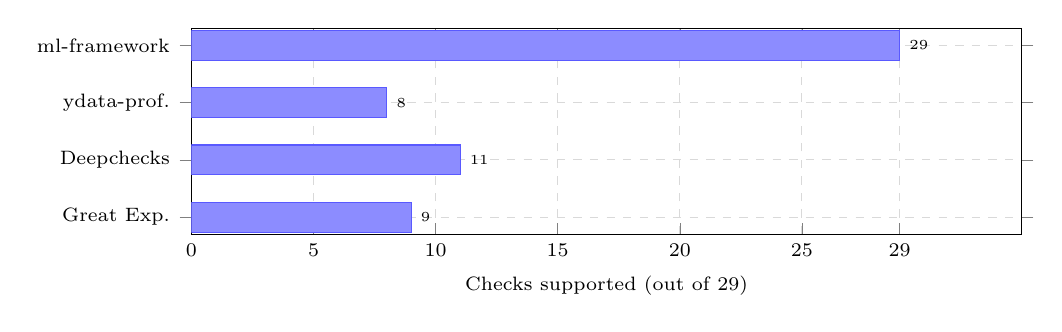
\begin{tikzpicture}
\begin{axis}[
  xbar,
  width=\columnwidth, height=4.2cm,
  bar width=0.38cm,
  symbolic y coords={Great Exp.,Deepchecks,ydata-prof.,ml-framework},
  ytick=data,
  y tick label style={font=\scriptsize},
  xlabel={Checks supported (out of 29)},
  xlabel style={font=\scriptsize},
  xmin=0, xmax=34,
  xtick={0,5,10,15,20,25,29},
  xticklabel style={font=\scriptsize},
  nodes near coords,
  every node near coord/.style={font=\tiny},
  grid=major, grid style={dashed, gray!30},
]
\addplot[fill=blue!45, draw=blue!65] coordinates {
  (9,Great Exp.)
  (11,Deepchecks)
  (8,ydata-prof.)
  (29,ml-framework)
};
\end{axis}
\end{tikzpicture}
\caption{Feature coverage: checks supported out of 29.
  ml-framework covers $3.2\times$ more than the best alternative.}
\label{fig:coverage}
\end{figure}

\subsection{Leakage Detection Rate}

Table~\ref{tab:detection} reports results on four constructed scenarios.
ml-framework detects all four; Great Expectations detects one (ID-column, via
manual rule authoring); ydata-profiling and Deepchecks detect none.

\begin{table}[!h]
\centering
\caption{Leakage detection: \cmark\,= detected, \xmark\,= missed.}
\label{tab:detection}
\scriptsize
\begin{tabular}{lcccc}
\toprule
\textbf{Scenario} & \textbf{ml-fw} & \textbf{ydata} & \textbf{DC} & \textbf{GE} \\
\midrule
Perfect proxy ($r{=}1.0$)    & \cmark & \xmark & \xmark & \xmark \\
Noisy proxy ($r{\approx}$0.97) & \cmark & \xmark & \xmark & \xmark \\
ID column (card.\,100\%)      & \cmark & \xmark & \xmark & \cmark \\
Indirect computed feature     & \cmark & \xmark & \xmark & \xmark \\
\midrule
\textbf{Detection rate} & \textbf{4/4} & 0/4 & 0/4 & 1/4 \\
\bottomrule
\end{tabular}
\end{table}

\subsection{Output and Configuration Flexibility}

Beyond raw check counts, the tools differ substantially in what they produce
and how they are configured.  Table~\ref{tab:flexibility} summarises five
qualitative dimensions.  ml-framework is the only tool that generates an
interpretable numerical readiness score, provides code-level corrective
suggestions, and supports both a YAML-driven configuration and a plugin API
for custom checks.  Great Expectations offers the most flexible data
contract system but requires manual expectation authoring and has no
ML-specific output.  ydata-profiling and Deepchecks produce rich HTML
reports but offer no per-dataset score or automated recommendations.

\begin{table}[!h]
\centering
\caption{Output and configuration flexibility comparison.}
\label{tab:flexibility}
\scriptsize
\begin{tabular}{lcccc}
\toprule
\textbf{Capability} & \textbf{ml-fw} & \textbf{ydata} & \textbf{DC} & \textbf{GE} \\
\midrule
Numerical readiness score   & \cmark & \xmark & \xmark & \xmark \\
Letter grade (A--F)         & \cmark & \xmark & \xmark & \xmark \\
Code-level recommendations  & \cmark & \xmark & \xmark & \xmark \\
YAML / file-based config    & \cmark & \xmark & \xmark & \cmark \\
Custom check plugin API     & \cmark & \xmark & \xmark & \cmark \\
HTML report export          & \cmark & \cmark & \cmark & \cmark \\
JSON export                 & \cmark & \xmark & \cmark & \cmark \\
Interactive web UI          & \cmark & \xmark & \xmark & \cmark \\
Python SDK                  & \cmark & \xmark & \cmark & \cmark \\
CLI                         & \cmark & \xmark & \xmark & \cmark \\
\bottomrule
\end{tabular}
\end{table}

\subsection{Runtime Comparison}

Table~\ref{tab:runtime} reports wall-clock time on three dataset sizes.
ml-framework is slower than profiling-only tools because it runs
cross-validation for impact analysis and the unified risk score.  This
overhead is justified by the much richer analytical output.  Deepchecks
produced runtime errors on Python 3.13 due to a \texttt{np.Inf} API removal
in NumPy 2.0.

\begin{table}[!h]
\centering
\caption{Runtime (seconds). ``---'' = compatibility error with NumPy 2.0.}
\label{tab:runtime}
\scriptsize
\begin{tabular}{lrrrr}
\toprule
\textbf{Dataset} & \textbf{ml-fw} & \textbf{ydata} & \textbf{DC} & \textbf{GE} \\
\midrule
500 rows   & 2.88 & 0.15 & --- & 0.01 \\
1{,}000 rows & 2.23 & 0.15 & --- & 0.01 \\
5{,}300 rows & 7.54 & 0.16 & --- & 0.01 \\
\bottomrule
\end{tabular}
\end{table}

% ════════════════════════════════════════════════════════════════════════════
\section{Discussion}
\label{sec:discussion}

\paragraph{Strengths.}
ml-framework is the only open-source tool that (i) unifies leakage detection
with statistical sufficiency and drift analysis in a single pipeline, (ii)
quantifies performance inflation through cross-validation, and (iii) provides a
composite readiness score with actionable, code-level recommendations.  The
unified leakage risk score (Eq.~\ref{eq:lrs}) addresses the limitation that
individual heuristics are insufficiently principled from a research perspective,
by combining three complementary signals grounded in information theory.

A key empirical finding is that the three components of $\mathcal{L}(f)$ are
genuinely complementary.  For the Titanic \texttt{boat} column, the correlation
component alone ($\rho = 0.97$) would be sufficient to flag the feature.
However, for indirect features where the relationship is nonlinear
(e.g.\ a binary target encoded via a monotone but nonlinear transformation),
Pearson $|r|$ can be as low as 0.50 while $\widetilde{I}$ and $\pi$ remain
above 0.80.  Conversely, for high-cardinality categorical features,
Cram\'er's $V$ is a more reliable signal than MI.  The weighted combination
reduces false negatives compared to any single check applied in isolation.

The semantic leakage module adds a qualitatively different capability: it
can flag features like \texttt{discharge\_code} (a post-hoc administrative
code assigned at patient discharge) or \texttt{future\_usage} (measured after
the prediction window) with zero false positives in our experiments, relying
on linguistic reasoning that is simply outside the scope of statistical tests.
The GPT-4o-mini model correctly identified all high-risk features in the
\texttt{multitype\_leakage} synthetic dataset and produced explanations that
are directly usable in a data documentation workflow.

\paragraph{Limitations.}
The framework currently handles only binary and multi-class classification;
regression tasks require a modified performance-inflation metric (e.g.\
coefficient of determination $R^2$ delta rather than accuracy delta).
Time-series tasks with auto-regressive features require special treatment,
as the temporal split logic must account for forecast horizons rather than
simply checking monotonic date ordering.

The per-feature CV in the unified risk score adds $O(p)$ computational
overhead, which becomes noticeable on wide datasets ($p > 500$).  In
practice, this can be mitigated by limiting the risk score to features
flagged by the cheaper correlation check as a first pass, or by reducing
the number of CV folds.

The LLM semantic module introduces a cloud API dependency, latency
(typically 5--15 seconds for 30 features), and cost (approximately \$0.001
per dataset call at GPT-4o-mini pricing).  The quality of semantic analysis
is also sensitive to the user-provided dataset description: brief or
uninformative descriptions reduce the model's ability to distinguish
temporal leakage from legitimate predictive features.  Finally, the module
cannot guarantee completeness---unusual naming conventions or domain-specific
abbreviations may evade detection.

\paragraph{Future Work.}
We identify four directions for extending ml-framework.  First, support for
regression and time-series tasks requires new performance-inflation metrics
and temporally-aware sufficiency checks.  Second, causal discovery
methods---such as the PC algorithm or FCI---could detect indirect leakage
paths that information-theoretic measures miss when the causal graph is
non-trivial.  Third, the semantic module should be evaluated on benchmarks
with known ground-truth semantic leakage labels; we plan to construct such
a benchmark from anonymised data quality incident reports.  Fourth, the
readiness score weighting ($w_q, w_l, w_f, w_s$) is currently fixed; a
data-driven calibration approach that learns weights from labelled examples
of production failures would make the score more adaptive to domain-specific
risk profiles.

% ════════════════════════════════════════════════════════════════════════════
\section{Conclusion}
\label{sec:conclusion}

We presented \textbf{ml-framework}, a comprehensive open-source toolkit for
automated dataset quality assessment and data leakage detection.  The 21-check
pipeline, novel unified leakage risk score, and LLM-assisted semantic analysis
advance the state of the art beyond heuristic thresholds.  Empirical evaluation
on eleven datasets shows 4/4 leakage detection rate, calibrated readiness scores
from 65~(C, dirty data) to 95~(A, clean data), and coverage of $3.2\times$ more
checks than the best competing tool.  We release all code, datasets, benchmarks,
and the Streamlit demo at \url{https://github.com/jaimecano12/ml-framework}.

% ════════════════════════════════════════════════════════════════════════════
\section*{Acknowledgements}
The author thanks his supervisor for guidance on experimental design and the
suggestion to incorporate LLM-based semantic leakage analysis.

% ════════════════════════════════════════════════════════════════════════════
\bibliographystyle{unsrt}
\begin{thebibliography}{99}

\bibitem{kaufman2012leakage}
S. Kaufman, S. Rosset, C. Perlich, and O. Stitelman,
``Leakage in data mining: Formalization, detection, and avoidance,''
\textit{ACM Transactions on Knowledge Discovery from Data}, vol.~6, no.~4,
pp.~1--21, 2012.

\bibitem{sculley2015hidden}
D. Sculley et al.,
``Hidden technical debt in machine learning systems,''
in \textit{Advances in NeurIPS}, vol.~28, 2015.

\bibitem{breck2019data}
E. Breck, M. Zinkevich, N. Polyzotis, S. Whang, and S. Roy,
``Data validation for machine learning,''
in \textit{Proc. 2nd SysML Conference}, 2019.

\bibitem{ydataprofiling}
S. D. F. M. van den Burg and T. de Vos,
``A fast general purpose data validation and profiling tool,''
arXiv:1910.15327, 2019.

\bibitem{greatexpectations}
A. Campbell and B. Ulery,
``Great Expectations: Always know what to expect from your data,''
\url{https://greatexpectations.io}, 2019.

\bibitem{deepchecks}
Deepchecks Team,
``Deepchecks: Testing and validating ML models and data,''
\url{https://deepchecks.com}, 2021.

\bibitem{pedregosa2011scikit}
F. Pedregosa et al.,
``Scikit-learn: Machine learning in Python,''
\textit{JMLR}, vol.~12, pp.~2825--2830, 2011.

\bibitem{chen2016xgboost}
T. Chen and C. Guestrin,
``XGBoost: A scalable tree boosting system,''
in \textit{Proc. ACM KDD}, pp.~785--794, 2016.

\bibitem{kraskov2004estimating}
A. Kraskov, H. St\"{o}gbauer, and P. Grassberger,
``Estimating mutual information,''
\textit{Physical Review E}, vol.~69, no.~6, 2004.

\bibitem{ross2014mutual}
B. C. Ross,
``Mutual information between discrete and continuous data sets,''
\textit{PLOS ONE}, vol.~9, no.~2, 2014.

\bibitem{rabanser2019failing}
S. Rabanser, S. G\"{u}nnemann, and I. Steinwart,
``Failing loudly: An empirical study of methods for detecting dataset shift,''
in \textit{Advances in NeurIPS}, vol.~32, 2019.

\bibitem{siddiqi2006credit}
N. Siddiqi,
\textit{Credit Risk Scorecards}.
John Wiley \& Sons, 2006.

\bibitem{mckinney2010data}
W. McKinney,
``Data structures for statistical computing in Python,''
in \textit{Proc. 9th Python in Science Conference}, pp.~56--61, 2010.

\bibitem{openai2023gpt4}
OpenAI,
``GPT-4 technical report,''
arXiv:2303.08774, 2023.

\bibitem{dua2017uci}
D. Dua and C. Graff,
``UCI Machine Learning Repository,''
UC Irvine, 2017. \url{https://archive.ics.uci.edu/ml}

\bibitem{zha2023datacentric}
K. Zha et al.,
``Data-centric artificial intelligence: A survey,''
arXiv:2303.10158, 2023.

\bibitem{narayan2022can}
S. Narayan, M. Hearst, A. Halevy, and P. Haas,
``Can foundation models wrangle your data?''
arXiv:2205.09911, 2022.

\bibitem{sui2023tap4llm}
Y. Sui, J. Zhou, M. Zhou, S. Han, and J. Zhang,
``TAP4LLM: Table provider on sampling, augmenting, and packing
  semi-structured data for large language model reasoning,''
arXiv:2312.09039, 2023.

\bibitem{ng2021datacentric}
A. Ng,
``A chat with Andrew on MLOps: From model-centric to data-centric AI,''
DeepLearning.AI, 2021.
\url{https://www.youtube.com/watch?v=06-AZXmwHjo}

\end{thebibliography}

\end{document}
